
%-----------------------------------
% ANNOTATING READINGS
%-----------------------------------


\chapter{Annotation \& Critical Reading}

\begin{quote} \small There is something predatory, cruel even, about a pen
suspended over a text. Like a hawk over a field, it is on the lookout for
something vulnerable. Then it is a pleasure to swoop and skewer the victim with
the nib’s sharp point. The mere fact of holding the hand poised for action
changes our attitude to the text. We are no longer passive consumers of a
monologue but active participants in a dialogue.

\textemdash Tim Parks,
"\href{http://www.nybooks.com/blogs/nyrblog/2014/dec/03/weapon-for-readers/}{A
Weapon for Readers}"

\end{quote}

In college you will encounter demanding texts of great complexity. You will be
asked to engage these texts critically and to challenge the thinking and conclusions of others. You will also have to retain an extraordinary amount of information and recall it later. To thrive in this environment you will need to develop some new habits and strategies. The most basic, and most important, of these are a formal procedure for the \textbf{annotation of texts} and the creation of \textbf{critical summary notes}. 

\section{Annotating texts}

Analysis requires breaking an argument down into smaller parts so that you can
understand how those parts work together to make the whole. The best way to
begin this process is to annotate texts as you read them by using a system of symbols and marginal notes made on the document itself. There is no right or wrong way to mark up a text, but you should develop
a system that you are comfortable with and try to stick with it. Writing while
you read will help you stay focused and read critically. In fact, I would argue
that if you are not writing while you read\textemdash by putting it into your
own words through annotation, \hyperlink{summary}{\color{Ahrenge}{summary}}, \hyperlink{paraphrase}{\color{Ahrenge}{paraphrase}}, and \hyperlink{quotation}{\color{Ahrenge}{quotation}}\textemdash then you are not reading critically at all.

Your objective in annotation is to flag the key elements of a piece of
writing\textemdash such as the thesis, argumentative points, and key pieces of
evidence. This kind of work serves two purposes. First, it helps you maintain a
critical focus as you read. Second, it helps you later if the text must be used for study or your own writing.

During my annotations, I try to flag a number of
things. I always underline the thesis once I find it and I place a large dot
next to pieces of evidence or statements being used to support the
thesis. I always place keywords or a short statement next to each paragraph,
aiming to create a "micro summary" of the content. I use check marks or
exclamation points next to statements that I find important or noteworthy.
Sometimes I draw arrows to connect parts of the essay that seem related to me in
some way.

In addition to flagging and summarizing a text's ideas and arguments, I also ask
questions in the margins or note places where I become confused. This is helpful
later, on my second reading, since I can pay more careful attention to the
passages that gave me trouble. I also write my thoughts as they occur to me and
state objections to things that seem problematic or wrongheaded. Sometimes I try
to connect an idea in one text with the idea(s) in another text I have read.
Thus, I may find places where I can compare/contrast the thinking of two or more
writers.

As you can see from the example here to the right, the process of annotation
keeps me engaged, active, and alert\textemdash key components in critical
thinking.

\begin{center} 
\begin{figure}
\href{https://github.com/stockphrase/OpenHandbook/blob/master/Chapters/images/Annotation1.jpg?raw=true}{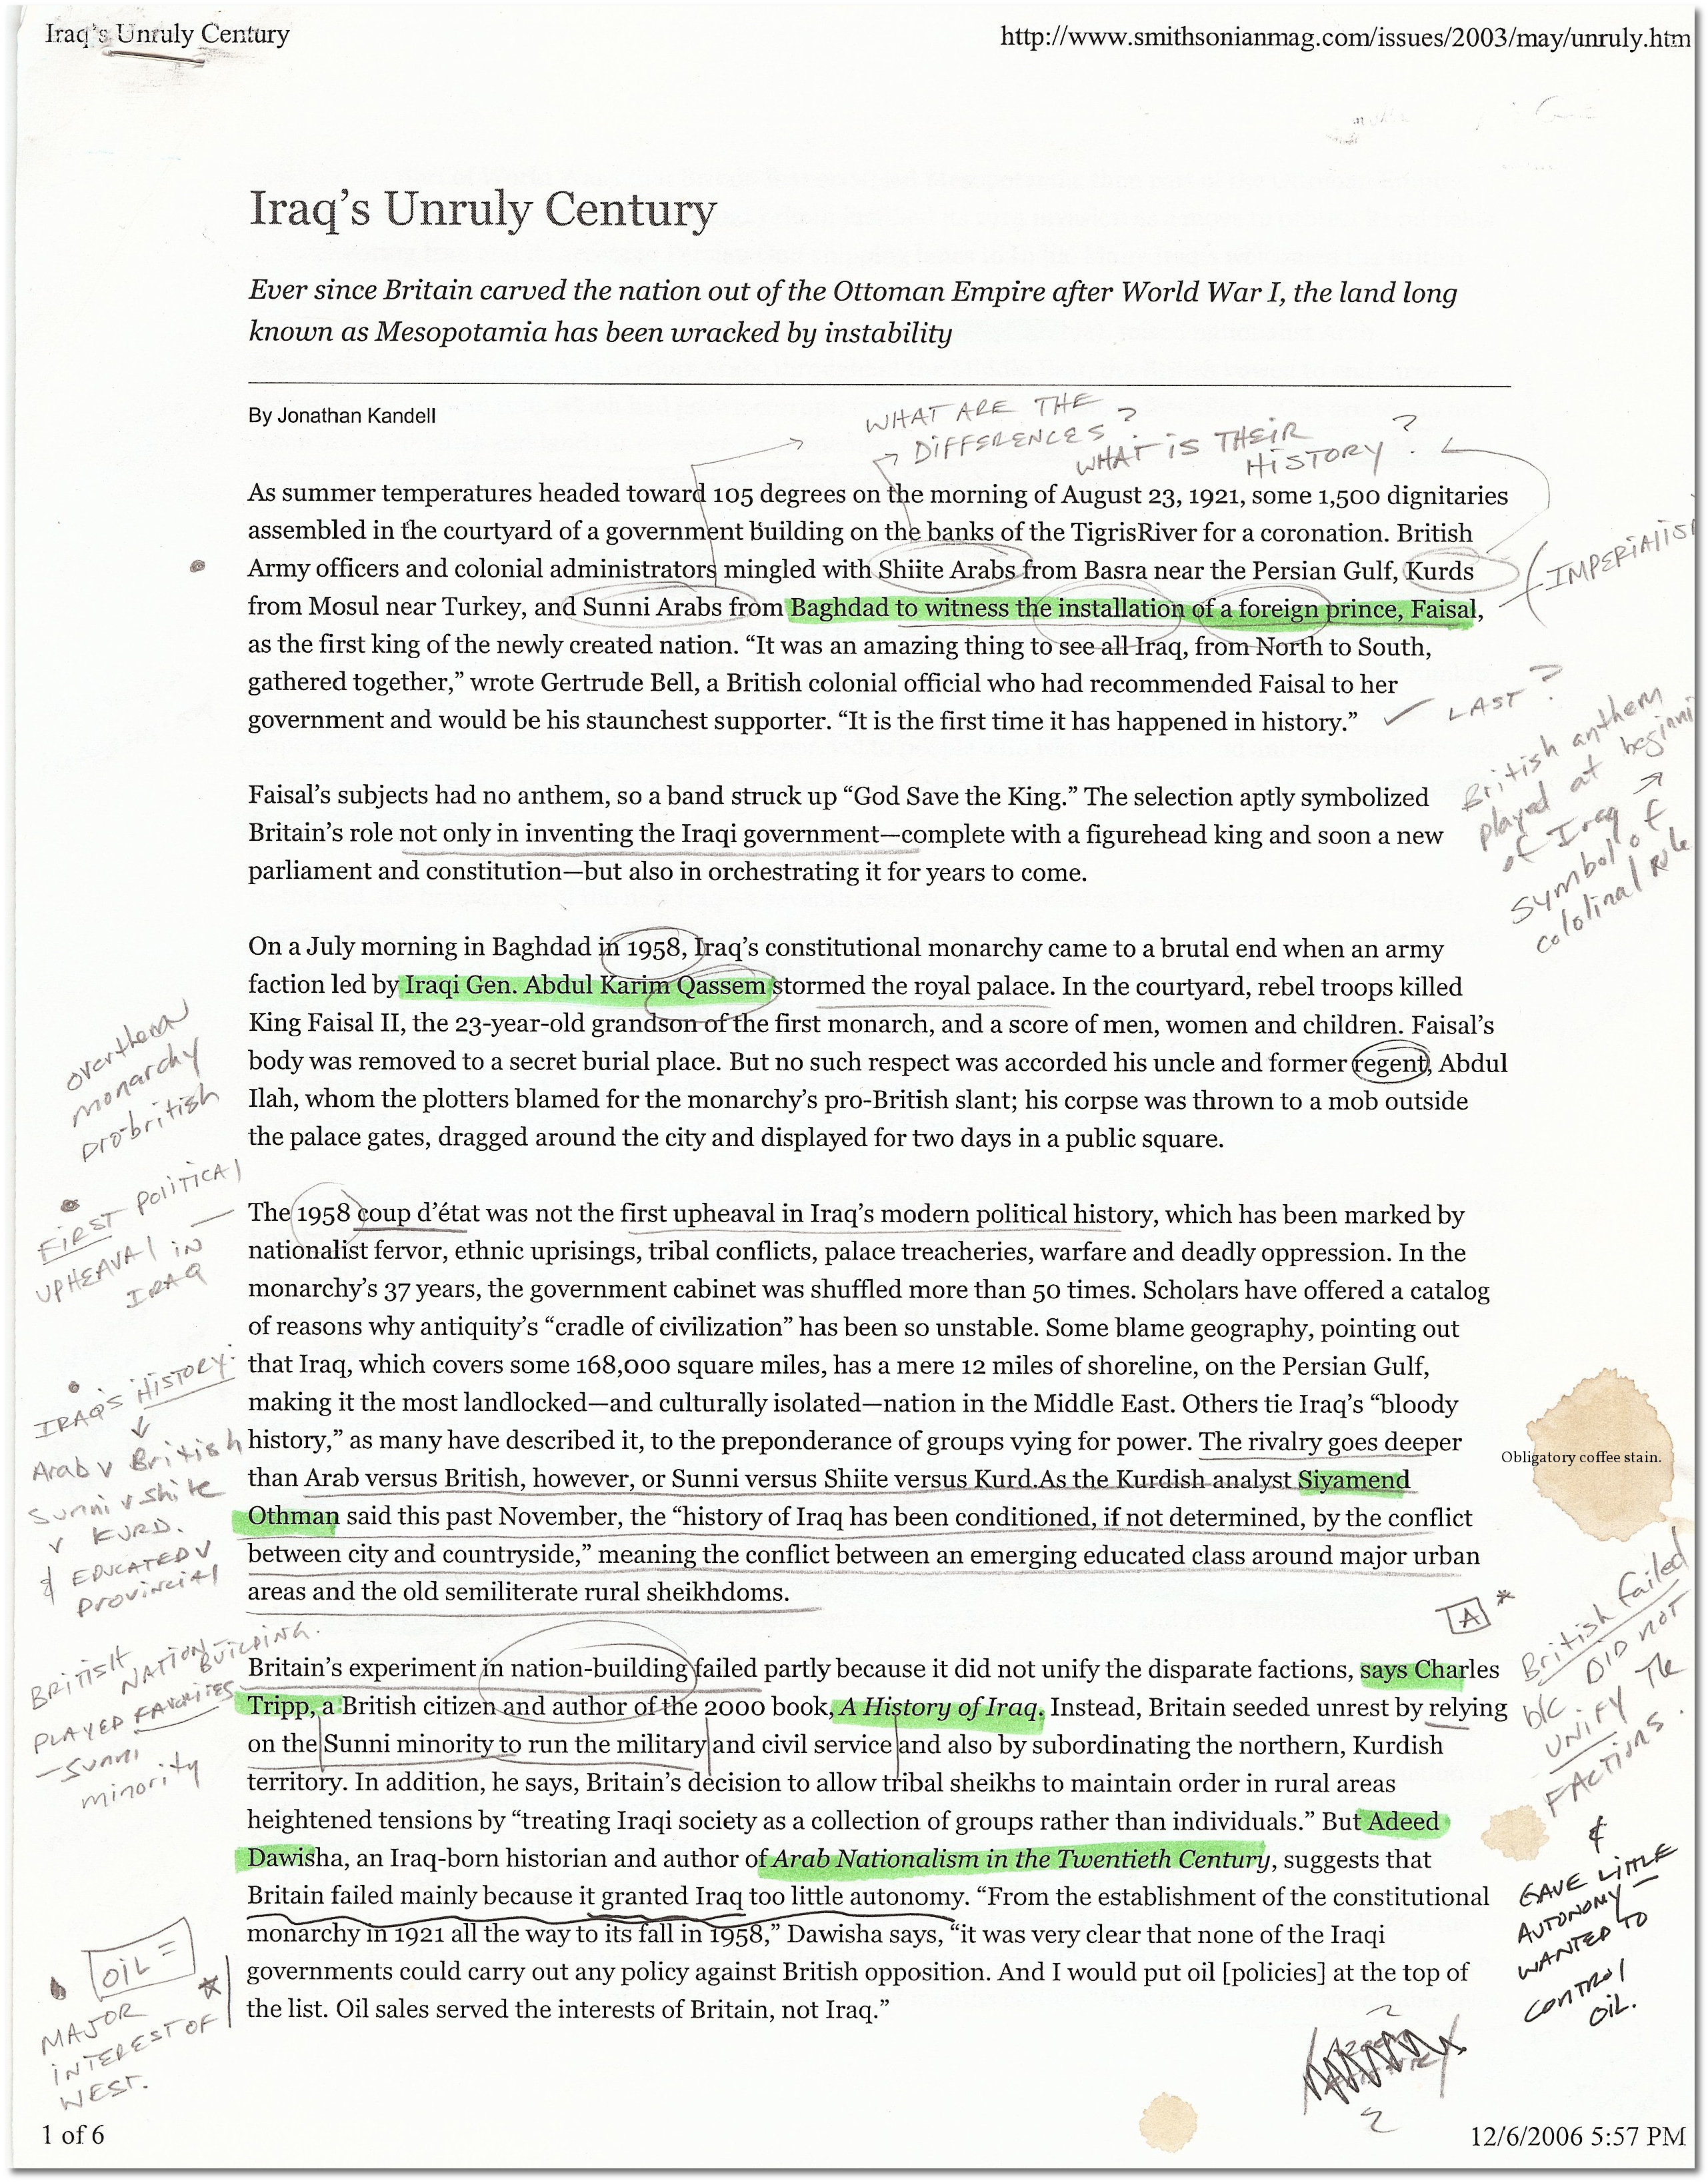
\includegraphics[scale=.135]{Annotation1.jpg}}
\end{figure}

%\href{https://github.com/stockphrase/OpenHandbook/blob/master/Chapters/images/Annotation1.jpg?raw=true}{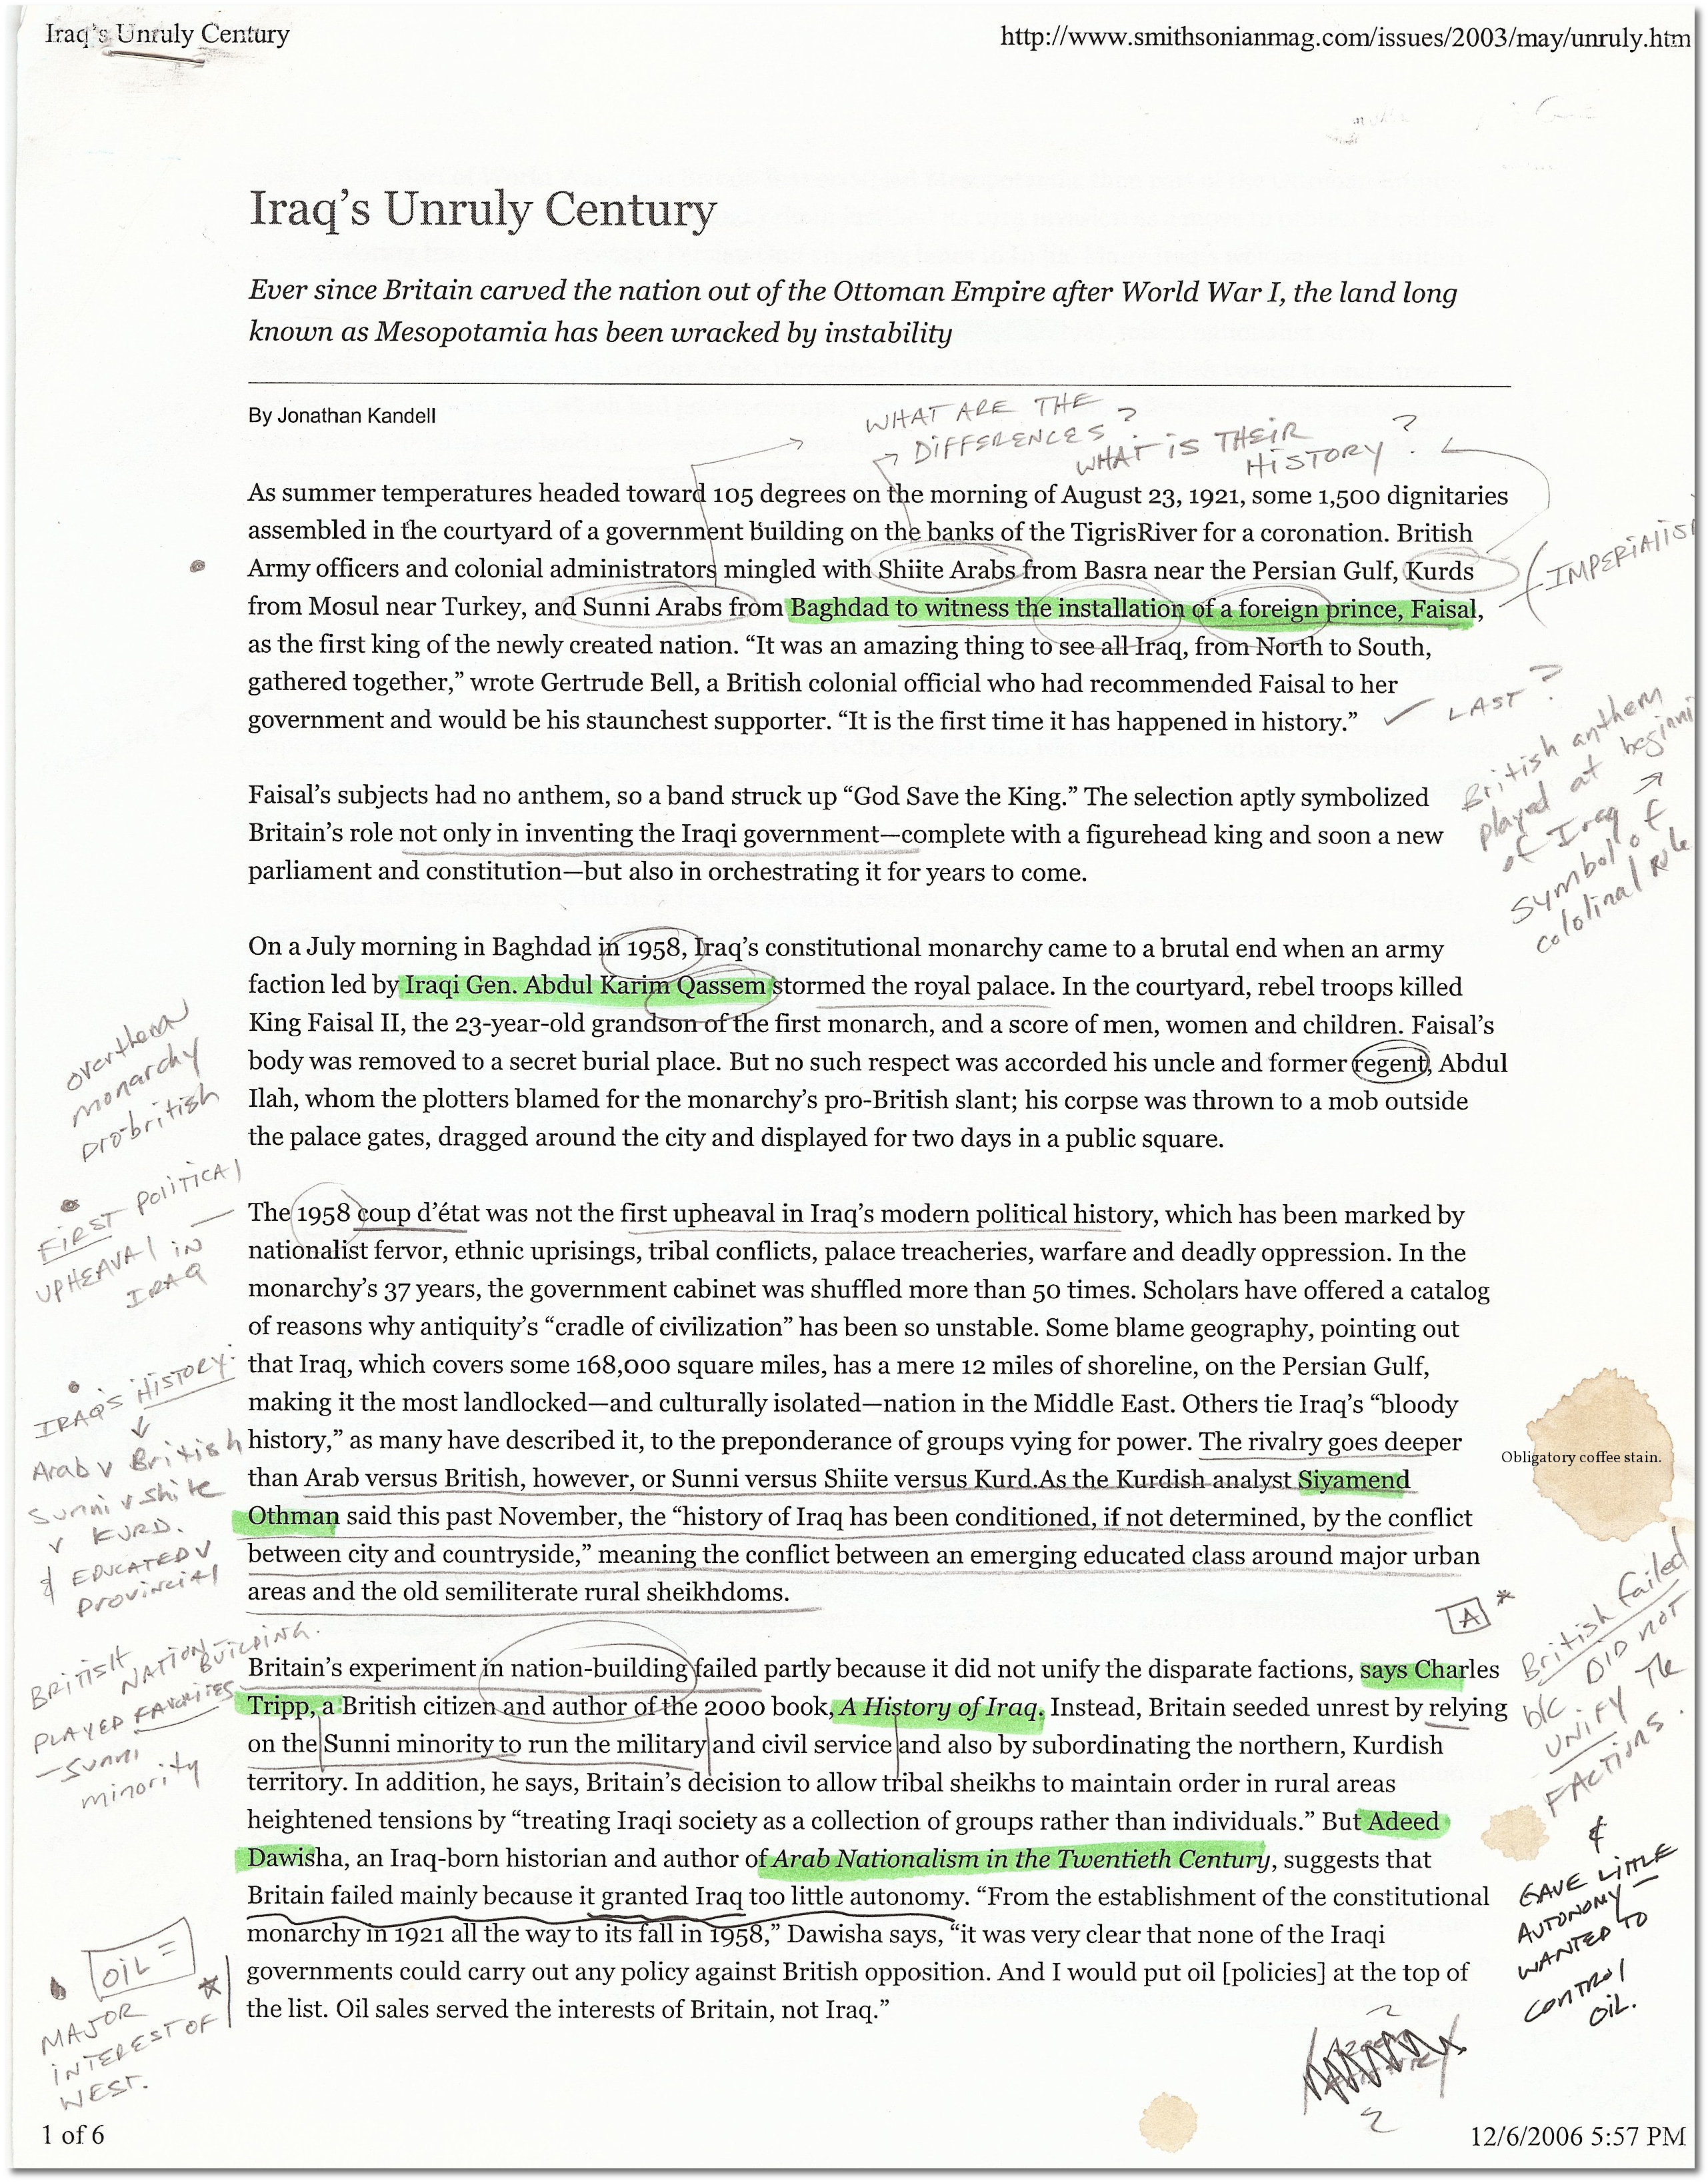
\includegraphics[scale=.135]{Annotation1.jpg}}


\end{center}



\subsection{The false allure of the highlighter}

Students often associate critical thinking and a general studiousness with the use of a highlighter. However, I'd like to question this practice a bit. Compare the following selection from a student's course reading to the annotation practices outlined above:

\bigskip

\begin{tcolorbox}[enhanced,width=4.2in,left=.4in, right=.4in,
   drop fuzzy shadow southeast,
    boxrule=0.4pt,sharp corners,colframe=black!80!black,colback=white!10]

\smallskip

\begin{flushright}

%\rule{4cm}{.7pt}

{\economica \emph{Biosystems} 31 (1993) \hspace{6pt} 238}

\end{flushright}

{\small
\begin{doublespacing}

\hspace{.5cm}At the heart of the environmentalist worldview is the conviction that \hl{human physical and spiritual health depends on sustaining the planet in a relatively unaltered state}. \hl{Earth is our home in the full, genetic sense,} where humanity and its ancestors existed for all the millions of years of their evolution. \hl{Natural ecosystems\textemdash forests, coral reefs, marine blue waters\textemdash maintain the world exactly as we would wish it to be maintained.} Our body and our mind evolved precisely to live in this particular planetary environment and no other. \hl{When we debase the global environment and extinguish the variety of life, we are dismantling a support system that is too complex to understand, let alone replace}, in the foreseeable future. . . . We run the risk, conclude the environmentalists, of beaching ourselves upon alien shores like a great confused pod of pilot whales.

\bigskip


\end{doublespacing}}

\end{tcolorbox}

There are a number of problems worth noting here about the practice of highlighting while reading: 

\begin{itemize}

\item First, your objective when you read something should be \emph{to avoid having to read it again} (unless, of course, you would enjoy doing so). Highlighting important portions of a text, as this student has done, only signals that the highlighted bits were important to the reader at the time of the reading. But to discover \emph{why} they are important or \emph{what} the highlighted portions mean, the student will be forced to read the text again. Busy students studying for multiple midterms do not have time to re-read entire books or articles.  

\item Secondly, highlighting works against critical thinking by casting the reader in the passive role of information consumer. As \href{http://libcat.dartmouth.edu/record=6773185}{Keith Hjortshoj argues}, highlighting merely "emphasizes the authority of the text: what its author says, believes, or knows. The practice therefore leads you toward memorization and repetition, not toward interpretation, inquiry, or criticism" (41). While recalling information at a later time is important, this is not the sole purpose of reading. Critical reading also involves a process of evaluating, questioning, and interpreting the text\textemdash activities that highlighting severely limit.

\item Thirdly, highlighting doesn't help you place the information into your long-term memory. \href{https://sites.udel.edu/victorp/files/2010/11/Psychological-Science-2014-Mueller-0956797614524581-1u0h0yu.pdf}{Recent empirical 
research} suggests that \href{https://www.scientificamerican.com/article/a-learning-secret-don-t-take-notes-with-a-laptop/}{taking notes by hand} results in a significant boost to information retention.

\item Finally, highlighting doesn't help you understand the structure of an argument\textemdash the main goal of any critical analysis. Arguments all have a certain structure: there is a main idea supported by a series of claims, reasons, and pieces of supporting evidence. The highlighter \emph{fails to reveal this structure}. Flagging key structural features of arguments, as described above in the process of annotation, will dramatically reduce the time it takes to study and will be of significant help in your writing as you make use of, or react to, the text.

\end{itemize}

\subsection{Annotation strategies}

Since you have likely never engaged a text in such a manner, here are some
strategies that you might consider as you develop a process for annotation and
critical reading:

\begin{itemize} \item \hloy{Use a symbol system}. Develop a system of symbols
to flag important aspects of a reading. Mark significant elements within the
text such as the thesis, argumentative claims, and evidence. Also note when a
text references other texts, authors, or events. Note places where you become
confused or uncertain; later, in a second reading, you can give extra attention
to these portions of the text.

\item \hloy{Interrogate the text}. Be ruthless. Be rigorous. Ask questions
back to the author in the margins of the text. Challenge the conclusions and
arguments that he or she presents by making ones of your own.

\item \hloy{Summarize}. Write keywords or make "microsummaries" in the margins
next to each paragraph. Later, you will not have to re-read the entire document
to find your place. These can be especially useful if you later use this text in
your own writing.

\item \hloy{Connect}. Find connections between the reading and others within
the course or your broader reading experience. Develop the capacity to bring
other texts into dialogue with each other, imagining writing and reading as a
form of social interaction. \end{itemize}



\chapter{Critical Notes}
\hypertarget{notes}{}

\begin{quote} \small "We believe the best way to work on a difficult text is by
rereading . . . but you can also work on the difficult text by writing, by taking
possession of the work through sentences and paragraphs of your own, through
summary, paraphrase, and quotation, by making another writer’s work part of your
work" (12).

\textemdash Bartholomae and Petrosky, "Introduction." \emph{Ways of Reading: An
Anthology for Writers}

\end{quote}

\section{Taking Critical Notes}

One objective of the annotations described in the previous chapter is to help you \textbf{create a
critical outline} during a subsequent reading. The objective in the critical
outline is to boil the entire argument down to its essence, without losing any
significant detail. The name of the game here is \textbf{reduction}: take
something large and unwieldy and turn it into something small and useful for
study or your own writing. There is a real art to this, and you will become
better and faster at this as you practice. Over time, you will train your mind
to operate in such a way that you will perform these tasks almost unconsciously
as you read. These critical notes will be indispensable study aids. They will
also dramatically improve and your writing.

These critical summaries are comprised of nothing more than \hyperlink{summary}{\color{Ahrenge}{summary}}, \hyperlink{paraphrase}{\color{Ahrenge}{paraphrase}}, \hyperlink{quotation}{\color{Ahrenge}{quotation}}, and your own observations and
questions. Quote only the most important, memorable language. Summarize or
paraphrase the rest in as objective a manner as possible. Take great care when
summarizing or paraphrasing; if your work is too similar to the original text
and is used later in your own writing, \emph{you may inadvertently commit
\hyperlink{plagiarism}{\color{Ahrenge}{plagiarism}}}, a serious academic
offense. Therefore, carefully place the writing of others into your own words
and cite the page numbers you reference in your notes.

As you write this critical outline you will not only try to reduce the main
points of the argument, you will also ask questions and make observations of the
text. You should note the argumentative points that you find yourself strongly
agreeing or disagreeing with and your reasons for doing so. You might see a
logical inconsistency or want the author to provide more evidence for his or her
claims. You might make a note to perform some research at the library or on the
Internet on an unfamiliar concept or event mentioned in the argument.
Ultimately, however, you will want to determine if the argument you have read is
persuasive and provide the reasons why.

At the end of this process, you should have a simplified\textemdash but
objective and accurate\textemdash version of the essay that has been ruthlessly
cut down to its bare essentials as well as a number of critical observations,
questions, and ideas that have emerged in your process of reading. By the time
you reach this stage and read over your notes, you will have taken great strides
toward mastering the information or argument. Of course, if the text is difficult, you may have to repeat the process until you have a breakthrough. I cannot emphasize enough how helpful and important this process is. It will help you come to a greater understanding of the text’s claims and weaknesses while also activating your long-term memory. 

Finally, to be a successful student and scholar, you will need to \hyperlink{joyofreuse}{\color{Ahrenge}{create a system for organizing and retaining these annotations and notes}} for later use. You might use a series of organized folders on your computer or some kind of filing system in manila folders. Whatever works best for you. Retaining all of this hard work will be of great importance to you later, particularly as you engage in large \hyperlink{academicresearch}{\color{Ahrenge}{research}} projects. As I describe in the next chapter, being a scholar\textemdash or just a great student\textemdash involves reusing and re-purposing prior work and information. 
 
\smallskip

\begin{center}
\begin{tcolorbox}[colframe=oyster, coltitle=black, sharp corners, title=\ding{52} Note]

\href{https://sites.udel.edu/victorp/files/2010/11/Psychological-Science-2014-Mueller-0956797614524581-1u0h0yu.pdf}{New research} suggests that taking notes by hand, \href{https://www.scientificamerican.com/article/a-learning-secret-don-t-take-notes-with-a-laptop/}{rather than using a computer}, aids memory and improves student performance.

\end{tcolorbox}
\end{center}


\subsection{Critical notes strategies}

Developing a process for making critical notes is perhaps the most important new
habit you will need to be successful in college. Here are some strategies or
principles that may guide your efforts:

\begin{itemize} \item \hloy{Reduce}. Use \hyperlink{summary}{\color{Ahrenge}{summary}}, \hyperlink{paraphrase}{\color{Ahrenge}{paraphrase}}, and \hyperlink{quotation}{\color{Ahrenge}{quotation}} to reduce an argument to its bare
bones.

\item \hloy{Engage}. Grapple with the ideas and arguments in the text. Ask
questions and make observations. You should note the argumentative points that
you find yourself strongly agreeing or disagreeing with and your reasons for
doing so. You might see a logical inconsistency or want the author to provide
more evidence for his or her claims. You might make a note to perform some
research on an unfamiliar word, concept, or event mentioned in the argument.

\item \hloy{Protect yourself}. Be scrupulous when you \hyperlink{summary}{\color{Ahrenge}{summarize}} and \hyperlink{paraphrase}{\color{Ahrenge}{paraphrase}}
source materials in your notes by ensuring that you use your own language and
sentence structure. A lazy mistake at this stage may cost you dearly later if
you inadvertently \hyperlink{plagiarism}{\color{Ahrenge}{plagiarize}} material. Don't forget to meticulously cite the page numbers of all the information you include in your notes.

\item \hloy{Save your work.} You will need to \hyperlink{joyofreuse}{\color{Ahrenge}{create a system for organizing and retaining these annotations}} and notes for later use. You might use a series of organized folders on your computer or some kind of filing system in manila folders. Whatever works best for you. 

\end{itemize}
